         \chapter{Physical and chemical change}\fancyfoot[LO,RE]{Chemistry: Chemical change}
    \setcounter{figure}{1}
    \setcounter{subfigure}{1}
    \label{m38709*cid1}
            \section{Introduction}
            \nopagebreak
            \label{m38709} $ \hspace{-5pt}\begin{array}{cccccccccccc}   \end{array} $ \hspace{2 pt}\raisebox{-5 pt}{
\includegraphics[width=0.5cm]{col11305.imgs/summary_www.png}} {(section shortcode: P10056 )} \par 
      \label{m38709*id62175}Matter is all around us. The desks we sit at, the air we breathe and the water we drink are all examples of matter. But matter doesn't always stay the same. It can change in many different ways. In this chapter, we are going to take a closer look at \textbf{physical} and \textbf{chemical} changes that occur in matter.\par 
    \label{m38709*cid2}
            \subsection*{Physical changes in matter}
            \nopagebreak
      \label{m38709*id62200}A \textbf{physical change} is one where the particles of the substances that are involved in the change are not broken up in any way. When water is heated for example, the temperature and energy of the water molecules increases and the liquid water evaporates to form water vapour. When this happens, some kind of change has taken place, but the molecular structure of the water has not changed. This is an example of a \textsl{physical change}.\par 
      \label{m38709*id62556}$\mathrm{H}{}_{2}\mathrm{O}\left(\mathrm{l}\right)\to \mathrm{H}{}_{2}\mathrm{O}\left(\mathrm{g}\right)$
      \par 
      \label{m38709*id62600}Conduction (the transfer of energy through a material) is another example of a physical change. As energy is transferred from one material to another, the \textsl{energy} of each material is changed, but not its chemical makeup. Dissolving one substance in another is also a physical change.\par 
\label{m38709*fhsst!!!underscore!!!id76}
 \Definition{   \label{id2458225}Physical change } { \label{m38709*meaningfhsst!!!underscore!!!id76}
      A change that can be seen or felt, but that doesn't involve the break up of the particles in the reaction. During a physical change, the \textsl{form} of matter may change, but not its \textsl{identity}. A change in temperature is an example of a physical change. 
       } 

\label{m38709*id0209834} You can think of a physical change as a person who is standing still. When they start to move (start walking) then a change has occurred and this is similar to a physical change. \par 
      \label{m38709*id62640}There are some important things to remember about physical changes in matter:\par 
      \label{m38709*id62644}\begin{enumerate}[noitemsep, label=\textbf{\arabic*}. ] 
            \label{m38709*uid1}\item \textsl{Arrangement of particles}\newline
When a physical change occurs, the particles (e.g. atoms, molecules) may re-arrange themselves without actually breaking up in any way. In the example of evaporation that we used earlier, the water molecules move further apart as their temperature (and therefore energy) increases. The same would be true if ice were to melt. In the solid phase, water molecules are packed close together in a very ordered way, but when the ice is heated, the molecules overcome the forces holding them together and they move apart. Once again, the particles have re-arranged themselves, but have not broken up.
\label{m38709*eid2342}\nopagebreak\noindent{}
    \begin{equation}
    \mathrm{H}{}_{2}\mathrm{O}\left(\mathrm{s}\right)\to \mathrm{H}{}_{2}\mathrm{O}\left(\mathrm{l}\right)\tag{12.1}
      \end{equation}
Figure~12.1 shows this more clearly. In each phase of water, the water molecule itself stays the same, but the way the molecules are arranged has changed. Note that in the solid phase, we simply show the water molecules as spheres. This makes it easier to see how tightly packed the molecules are. In reality the water molecules would all look the same.
    \setcounter{subfigure}{0}
	\begin{figure}[H] % horizontal\label{m38709*uid2}
\begin{figure}[h]
\begin{center}
\begin{pspicture}(0,0)(10,2.6)
\SpecialCoor
%\psgrid[gridcolor=lightgray]
\def\water{\psset{unit=0.25}\rput{150}{\pscircle(0,0){2}
\psarc[fillcolor=white,fillstyle=solid](-1.5,1){1.5}{30}{260}
\psarc[fillcolor=white,fillstyle=solid](1.5,1){1.5}{280}{150}
\rput(-1.5,1){\pscurve(1.5;30)(-1;142.5)(1.5;260)}
\rput(1.5,1){\pscurve(1.5;150)(-1;37.5)(1.5;280)}}}

\rput(0,0.5){\psframe(0,0)(3,2)
\rput(0.25,0.4){\multirput(0.2,0.2)(0.4,0){6}{\pscircle(0,0){0.2}}
\multirput(0.2,0.6)(0.4,0){6}{\pscircle(0,0){0.2}}
\multirput(0.2,1)(0.4,0){6}{\pscircle(0,0){0.2}}
\multirput(0.4,0.8)(0.4,0){5}{\pscircle(0,0){0.1}}
\multirput(0.4,0.4)(0.4,0){5}{\pscircle(0,0){0.1}}}}


\rput(3.5,0){\psframe(0,0.5)(3,2.5)
\rput(1.5,1){\psset{unit=0.5}\rput(0,-0.2){\water}
\rput{185}(0,0.9){\water}
\rput{120}(2,1){\water}
\rput{310}(-2,1){\water}
\rput(0,2.4){\water}}}

\rput(7,0){\psframe(0,0.5)(3,2.5)
\rput(1.5,1){\psset{unit=0.5}\rput{120}(2,1){\water}
\rput{250}(-1,2){\water}}}

\uput[d](1.5,0.5){solid}
\uput[d](5,0.5){liquid}
\uput[d](8.5,0.5){gas}

\end{pspicture}
\end{center}
\caption{The arrangement of water molecules in the three phases of matter}
\label{fig:physical change:water phases}
\end{figure}
 \end{figure}       
\label{m38709*uid221}\item \textsl{Conservation of mass}\newline
    In a physical change, the total mass, the number of atoms and the number of molecules will always stay the same. In other words you will always have the same number of molecules or atoms at the end of the change as you had at the beginning. 
\label{m38709*uid3}\item \textsl{Energy changes}\newline
Energy changes may take place when there is a physical change in matter, but these energy changes are normally smaller than the energy changes that take place during a chemical change.
\label{m38709*uid4}\item \textsl{Reversibility}\newline
Physical changes in matter are usually easier to reverse than chemical changes. Water vapour for example, can be changed back to liquid water if the temperature is lowered. Liquid water can be changed into ice by simply decreasing the temperature.
\end{enumerate}
        \label{m38709*eip-904}\begin{activity}{Physical change}Use plastic pellets or marbles to represent water in the solid state. What do you need to do to the pellets to represent the change from solid to liquid? \par 
\end{activity}
    \label{m38709*cid3}
            \subsection*{Chemical Changes in Matter}
            \nopagebreak
      \label{m38709*id62778}When a \textbf{chemical change} takes place, new substances are formed in a chemical reaction. These new products may have very different properties from the substances that were there at the start of the reaction.\par 
      \label{m38709*id62788}The breakdown of copper (II) chloride to form copper and chlorine is an example of chemical change. A simplified diagram of this reaction is shown in Figure~12.2. In this reaction, the initial substance is copper (II) chloride, but once the reaction is complete, the products are copper and chlorine.\par 
    \setcounter{subfigure}{0}
	\begin{figure}[H] % horizontal\label{m38709*uid5}
\begin{figure}[h]
\begin{center}
\begin{pspicture}(-5,-1)(4.5,1.5)
%\psgrid[gridcolor=lightgray]
\psellipse(-3,0)(0.6,0.6)
\rput(-3,0){\textbf{Cu}}
\psellipse(-4,0)(0.4,0.4)
\rput(-4,0){\textbf{Cl}}
\psellipse(-2,0)(0.4,0.4)
\rput(-2,0){\textbf{Cl}}
\psline[arrows=->](-1,0)(0,0)
\psellipse(1,0)(0.6,0.6)
\rput(1,0){\textbf{Cu}}
\rput(2,0){\textbf{+}}
\psellipse(2.8,0)(0.4,0.4)
\rput(2.8,0){\textbf{Cl}}
\psellipse(3.6,0)(0.4,0.4)
\rput(3.6,0){\textbf{Cl}}
\end{pspicture}
\end{center}
\begin{center}
\rm${CuCl_{2} \rightarrow Cu + Cl_{2}}$
\end{center}
\caption{The decomposition of copper(II) chloride to form copper and chlorine}
\label{fig:physchem:cucl2}
\end{figure}
 \end{figure}       
\par
            \label{m38709*fhsst!!!underscore!!!id107}
 \Definition{   \label{id2458579}\textbf{ Chemical change }} { \label{m38709*meaningfhsst!!!underscore!!!id107}
      The formation of new substances in a chemical reaction. One type of matter is changed into something different. 
       } 
      \label{m38709*id62865}There are some important things to remember about chemical changes:\par 
      \label{m38709*id62869}\begin{enumerate}[noitemsep, label=\textbf{\arabic*}. ] 
            \label{m38709*uid6}\item \textsl{Arrangement of particles}\newline
During a chemical change, the particles themselves are changed in some way. In the example of copper (II) chloride that was used earlier, the $\mathrm{CuCl}{}_{2}$ molecules were split up into their component atoms. The number of particles will change because each $\mathrm{CuCl}{}_{2}$ molecule breaks down into one copper atom ($\mathrm{Cu}$) and one chlorine molecule ($\mathrm{CuCl}{}_{2}$). However, what you should have noticed, is that the number of atoms of each element stays the same, as does the total mass of the atoms. This will be discussed in more detail in a later section.
\label{m38709*uid7}\item \textsl{Energy changes}\newline
The energy changes that take place during a chemical reaction are much greater than those that take place during a physical change in matter. During a chemical reaction, energy is used up in order to break bonds, and then energy is released when the new product is formed. This will be discussed in more detail in "Energy changes in chemical reactions".
\label{m38709*uid8}\item \textsl{Reversibility}\newline
Chemical changes are far more difficult to reverse than physical changes.
\end{enumerate}
      \label{m38709*id62997}We will consider two types of chemical reactions: \textbf{decomposition reactions} and \textbf{synthesis reactions}.\par 
      \label{m38709*uid9}
            \subsubsection*{Decomposition reactions}
            \nopagebreak
            \label{m38709*id63019}A \textbf{decomposition reaction} occurs when a chemical compound is broken down into elements or smaller compounds. The generalised equation for a decomposition reaction is:\par 
        \label{m38709*id63029}$\mathrm{AB}\to \mathrm{A}+\mathrm{B}$\par 
        \label{m38709*id63040}One example of such a reaction is the decomposition of mercury (II) oxide (Figure~12.3) to form mercury and oxygen according to the following equation:
\label{m38709*id734}\nopagebreak\noindent{}

    \begin{equation}
    2\mathrm{HgO}\to 2\mathrm{Hg}+{\mathrm{O}}_{2}\tag{12.2}
      \end{equation}
    \setcounter{subfigure}{0}
	\begin{figure}[H] % horizontal\label{m38709*uid10}
    \begin{center}
    \label{m38709*uid10!!!underscore!!!media}\label{m38709*uid10!!!underscore!!!printimage}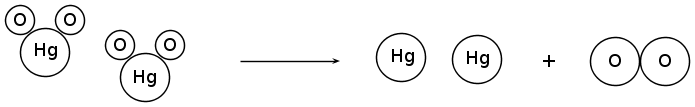
\includegraphics[width=300px]{col11305.imgs/m38709_CG10C4_003.png} % m38709;CG10C4\_003.png;;;6.0;8.5;
      \vspace{2pt}
    \vspace{\rubberspace}\par \begin{cnxcaption}
	  \small \textbf{Figure 12.3: }The decomposition of $\mathrm{HgO}$ to form $\mathrm{Hg}$ and ${\mathrm{O}}_{2}$
	\end{cnxcaption}
    \vspace{.1in}
    \end{center}
 \end{figure}       \par 
        \label{m38709*id63156}The decomposition of hydrogen peroxide is another example.\par 
\label{m38709*secfhsst!!!underscore!!!id163}
            \begin{g_experiment}{The decomposition of hydrogen peroxide}
            \nopagebreak
            \label{m38709*id63175}\noindent{}\textbf{Aim:}\newline
    To observe the decomposition of hydrogen peroxide when it is heated.\par 
        \label{m38709*id63194}\noindent{}\textbf{Apparatus:}\newline
    Dilute hydrogen peroxide (about 3\%); manganese dioxide; test tubes; a water bowl; stopper and delivery tube\par 
        \label{m38709*eip-470}
\Warning{Hydrogen peroxide can cause chemical burns. Work carefully with it.}
	\par
      \label{m38709*id63199}
    \setcounter{subfigure}{0}
	\begin{figure}[H] % horizontal\label{m38709*id63200}
    \begin{center}
    \label{m38709*id63200!!!underscore!!!media}\label{m38709*id63200!!!underscore!!!printimage}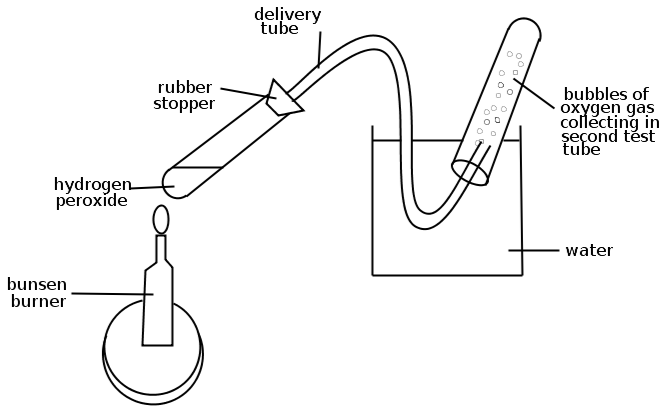
\includegraphics[width=300px]{col11305.imgs/m38709_CG10C4_004.png} % m38709;CG10C4\_004.png;;;6.0;8.5;
      \vspace{2pt}
    \vspace{.1in}
    \end{center}
 \end{figure}       
        \par 
        \label{m38709*id63206}\noindent{}\textbf{Method:}\label{m38709*id63212}\begin{enumerate}[noitemsep, label=\textbf{\arabic*}. ] 
            \label{m38709*uid11}\item Put a small amount (about 5 ml) of hydrogen peroxide in a test tube.
\label{m38709*uid12}\item Set up the apparatus as shown in Figure~12.4
\label{m38709*uid13}\item Very carefully add a small amount (about 0,5 g) of manganese dioxide to the test tube containing hydrogen peroxide. 
\end{enumerate}
        \par 
        \label{m38709*id63254}\noindent{}\textbf{Results:}\newline
    You should observe a gas bubbling up into the second test tube. This reaction happens quite rapidly. \par 
        \label{m38709*id63302}\noindent{}\textbf{Conclusions:}\newline
    When hydrogen peroxide is added to manganese dioxide it decomposes to form oxygen and water. The chemical decomposition reaction that takes place can be written as follows:
        \label{m38709*id63313}\nopagebreak\noindent{}
    \begin{equation}
    2{\mathrm{H}}_{2}{\mathrm{O}}_{2}\to 2\mathrm{H}{}_{2}\mathrm{O}+{\mathrm{O}}_{2}\tag{12.3}
      \end{equation}
Note that the manganese dioxide is a catalyst and is not shown in the reaction. (A catalyst helps speed up a chemical reaction.)    \par 
\end{g_experiment}
\label{m38709*eip-619}
\Note{The previous experiment used the downward displacement of water to collect a gas. This is a very common way to collect a gas in chemistry. The oxygen that is evolved in this reaction moves along the delivery tube and then collects in the top of the test tube. It does this because it is lighter than water and so displaces the water downwards. If you use a test tube with an outlet attached, you could collect the oxygen into jars and store it for use in other experiments.} 
	\par
      \label{m38709*eip-633}The above experiment can be very vigourous and produce a lot of oxygen very rapidly. For this reason you use dilute hydrogen peroxide and only a small amount of manganese dioxide. \par 
      \label{m38709*uid17}
            \subsubsection*{Synthesis reactions}
            \nopagebreak
            \label{m38709*id63365}During a \textbf{synthesis reaction}, a new product is formed from elements or smaller compounds. The generalised equation for a synthesis reaction is as follows:
        \label{m38709*id63374}\nopagebreak\noindent{}
    \begin{equation}
    \mathrm{A}+\mathrm{B}\to \mathrm{AB}\tag{12.4}
      \end{equation}
    \par 
        \label{m38709*id63386}One example of a synthesis reaction is the burning of magnesium in oxygen to form magnesium oxide(Figure~12.5). The equation for the reaction is:
        \label{m38709*id63390}\nopagebreak\noindent{}
    \begin{equation}
    2\mathrm{Mg}+{\mathrm{O}}_{2}\to 2\mathrm{MgO}\tag{12.5}
      \end{equation}
    \setcounter{subfigure}{0}
\begin{figure}[h]
\begin{center}
\begin{pspicture}(-6,-1)(6,1.5)
%\psgrid[gridcolor=lightgray]
\rput(-1,0){
\psellipse(-5,0)(0.75,0.75)
\rput(-5,0){Mg}
\psellipse(-3.2,0)(0.75,0.75)
\rput(-3.2,0){Mg}
\rput(-2,0){\textbf{+}}
\psellipse(-1,0)(0.5,0.5)
\rput(-1,0){O}
\psellipse(0,0)(0.5,0.5)
\rput(0,0){O}
\psline[arrows=->](1,0)(2.5,0)
\psellipse(3.5,0)(0.75,0.75)
\rput(3.5,0){Mg}
\psellipse(4.75,0)(0.5,0.5)
\rput(4.75,0){O}
\rput(3,0){
\psellipse(3.5,0)(0.75,0.75)
\rput(3.5,0){Mg}
\psellipse(4.75,0)(0.5,0.5)
\rput(4.75,0){O}
}
}
\end{pspicture}
\end{center}
\caption{The synthesis of magnesium oxide (MgO) from magnesium and oxygen}
\label{fig:chemical change:synthesis}
\end{figure}      \par 
\label{m38709*secfhsst!!!underscore!!!id243}
            \begin{g_experiment}{Chemical reactions involving iron and sulphur }
            \nopagebreak
            \label{m38709*id63437}\noindent{}\textbf{Aim:}
          \newline
     To demonstrate the synthesis of iron sulphide from iron and sulphur.\par 
        \label{m38709*id63447}\noindent{}\textbf{Apparatus:}
          \newline
5,6 g iron filings and 3,2 g powdered sulphur; porcelain dish; test tube; Bunsen burner\par 
        \label{m38709*id63457}
    \setcounter{subfigure}{0}
	\begin{figure}[H] % horizontal\label{m38709*id63460}
    \begin{center}
\begin{pspicture}(0,-4.301621)(6.4140625,4.253465)
\psline[linewidth=0.04cm](2.4714065,1.4040043)(4.351406,3.0040045)
\psline[linewidth=0.04cm](3.0114062,0.8440044)(4.811406,2.4440045)
\rput{-49.11223}(-0.46802804,4.402622){\psellipse[linewidth=0.04,dimen=outer](4.5838127,2.7134783)(0.3788815,0.19499093)}
\rput{130.79858}(5.409092,-0.2251927){\psarc[linewidth=0.04](2.7560983,1.125682){0.38911715}{0.0}{180.22943}}
\psline[linewidth=0.04cm](2.48,1.4134653)(3.66,1.3934652)
\rput{-50.467102}(-2.1400015,3.1871772){\psframe[linewidth=0.04,dimen=outer](2.7114062,4.004004)(1.911406,3.7240043)}
\psline[linewidth=0.04cm](2.611406,3.6040044)(2.7514062,3.424004)
\psline[linewidth=0.04cm](2.7514062,3.424004)(3.0114062,3.384004)
\psline[linewidth=0.04cm](3.0114062,3.384004)(3.5714064,2.6840045)
\psline[linewidth=0.04cm](3.5714064,2.6840045)(3.6314063,2.4440045)
\psline[linewidth=0.04cm](2.4914062,3.5040045)(2.611406,3.3640041)
\psline[linewidth=0.04cm](2.611406,3.3640041)(2.6314063,3.1840045)
\psline[linewidth=0.04cm](2.6314063,3.1840045)(2.6514063,3.1240041)
\psline[linewidth=0.04cm](2.6514063,3.1240041)(3.1714065,2.5040045)
\psline[linewidth=0.04cm](3.1714065,2.5040045)(3.9314063,2.0040045)
\psline[linewidth=0.04cm](3.9314063,2.0040045)(4.1114063,2.2240043)
\psline[linewidth=0.04cm](4.1114063,2.2240043)(3.4914062,2.5040045)
\psline[linewidth=0.04cm](3.4914062,2.5040045)(2.7914064,3.2240043)
\psline[linewidth=0.04cm](2.7914064,3.2240043)(2.6714065,3.2840044)
\psline[linewidth=0.04cm](2.7914064,3.2240043)(2.9914062,3.1840045)
\psline[linewidth=0.04cm](2.9914062,3.1840045)(3.4714065,2.664004)
\psline[linewidth=0.04cm](3.4714065,2.664004)(3.5314064,2.4840045)
\psline[linewidth=0.04cm](3.44,2.2134652)(3.4514065,1.9640043)
\psline[linewidth=0.04cm](3.4514065,1.9640043)(3.6914065,1.7640043)
\psline[linewidth=0.04cm](3.6914065,1.7640043)(3.9114063,1.9840044)
\psline[linewidth=0.04cm](3.9114063,1.9840044)(3.6714065,2.0840044)
\psline[linewidth=0.04cm](3.6714065,2.0840044)(3.56,2.2534652)
\pspolygon[linewidth=0.04](2.5914063,-0.07599564)(2.5914063,-0.61599565)(2.3714063,-0.7759956)(2.3114064,-2.2759957)(2.9114063,-2.2759957)(2.9114063,-0.7159956)(2.7714062,-0.55599564)(2.7714062,-0.07599564)
\rput{-204.0165}(3.8733587,-5.2158813){\psarc[linewidth=0.04](2.491407,-2.1959953){0.96}{301.69748}{268.90167}}
\rput{-204.0165}(3.7619426,-5.4846077){\psarc[linewidth=0.04](2.4642787,-2.342208){0.9778325}{0.77209437}{203.44756}}
\psellipse[linewidth=0.04,dimen=outer](2.6814063,0.24400435)(0.17,0.3)
\end{pspicture} 
    \end{center}
 \end{figure}       
        \par 
        \label{m38709*id63467}\noindent{}\textbf{Method:}
          \newline
        \label{m38709*id63473}\begin{enumerate}[noitemsep, label=\textbf{\arabic*}. ] 
            \label{m38709*uid20}\item Measure the quantity of iron and sulphur that you need and mix them in a porcelain dish.
\label{m38709*uid21}\item Take some of this mixture and place it in the test tube. The test tube should be about 1/3 full.
\label{m38709*uid22}\item This reaction should ideally take place in a fume cupboard. Heat the test tube containing the mixture over the Bunsen burner. Increase the heat if no reaction takes place. Once the reaction begins, you will need to remove the test tube from the flame. Record your observations.
\label{m38709*uid23}\item Wait for the product to cool before breaking the test tube with a hammer. Make sure that the test tube is rolled in paper before you do this, otherwise the glass will shatter everywhere and you may be hurt.
\label{m38709*uid24}\item What does the product look like? Does it look anything like the original reactants? Does it have any of the properties of the reactants (e.g. the magnetism of iron)?
\end{enumerate}
        \par 
        \label{m38709*eip-963}
      \Warning{When working with a bunsen burner work in a well ventilated space and ensure that there are no flammable substances close by. Always tuck loose clothing in and ensure that long hair is tied back.}
	\par
      \label{m38709*id63554}\noindent{}\textbf{Results:}
          \newline
        \label{m38709*id63560}\begin{enumerate}[noitemsep, label=\textbf{\arabic*}. ] 
            \label{m38709*uid25}\item After you removed the test tube from the flame, the mixture glowed a bright red colour. The reaction is exothermic and \textsl{produces energy}.
\label{m38709*uid26}\item The product, iron sulphide, is a dark colour and does not share any of the properties of the original reactants. It is an entirely new product.
\end{enumerate}
        \par 
        \label{m38709*id63594}\noindent{}\textbf{Conclusions:}
          \newline
A synthesis reaction has taken place. The equation for the reaction is:
        \label{m38709*id63604}\nopagebreak\noindent{}
    \begin{equation}
    \mathrm{Fe}+\mathrm{S}\to \mathrm{FeS}\tag{12.6}
      \end{equation}
    \par 
\end{g_experiment}
\label{m38709*secfhsst!!!underscore!!!id294}
            \begin{Investigation}{Physical or chemical change? }
            \nopagebreak
        \label{m38709*id63636}\noindent{}\textbf{Apparatus:}
Bunsen burner, 4 test tubes, a test tube rack and a test tube holder, small spatula, pipette, magnet, a birthday candle, $\mathrm{NaCl}$ (table salt), $0,1\phantom{\rule{2pt}{0ex}}\mathrm{M}\phantom{\rule{4pt}{0ex}}{\mathrm{AgNO}}_{3}$, $6\phantom{\rule{2pt}{0ex}}\mathrm{M}\phantom{\rule{4pt}{0ex}}\mathrm{HCl}$, magnesium ribbon, iron filings, sulphur.\par 
        \label{m38709*eip-118}
\Warning{${\mathrm{AgNO}}_{3}$ stains the skin. Be careful when working with it or use gloves.}
	\par
      \label{m38709*id62113}\noindent{}\textbf{Method:}
        \label{m38709*id62119}\begin{enumerate}[noitemsep, label=\textbf{\arabic*}. ] 
            \label{m38709*uid27}\item Place a small amount of wax from a birthday candle into a test tube and heat it over the bunsen burner until it melts. Leave it to cool.
\label{m38709*uid28}\item Add a small spatula of $\mathrm{NaCl}$ to 5 ml water in a test tube and shake. Then use the pipette to add 10 drops of ${\mathrm{AgNO}}_{3}$ to the sodium chloride solution. NOTE: Please be careful ${\mathrm{AgNO}}_{3}$ causes bad stains!!
\label{m38709*uid29}\item Take a 5 cm piece of magnesium ribbon and tear it into 1 cm pieces. Place two of these pieces into a test tube and add a few drops of $6\phantom{\rule{2pt}{0ex}}\mathrm{M}\phantom{\rule{4pt}{0ex}}\mathrm{HCl}$. NOTE: Be very careful when you handle this acid because it can cause major burns.
\label{m38709*uid30}\item Take about 0,5 g iron filings and 0,5 g sulphur. Test each substance with a magnet. Mix the two samples in a test tube and run a magnet alongside the outside of the test tube.
\label{m38709*uid31}\item Now heat the test tube that contains the iron and sulphur. What changes do you see? What happens now, if you run a magnet along the outside of the test tube?
\label{m38709*uid32}\item In each of the above cases, record your observations.
\end{enumerate}
        \par 
        \label{m38709*id63979}\noindent{}\textbf{Questions:}
Decide whether each of the following changes are physical or chemical and give a reason for your answer in each case. Record your answers in the table below:
    % \textbf{m38709*id63990}\par
          \begin{table}[H]
    % \begin{table}[H]
    % \\ '' '0'
        \begin{center}
      \label{m38709*id63990}
    \noindent
    \tabletail{%
        \hline
        \multicolumn{3}{|p{\mytableboxwidth}|}{\raggedleft \small \sl continued on next page}\\
        \hline
      }
      \tablelasttail{}
      \begin{xtabular}[t]{|l|l|l|}\hline
                  \textbf{Description}
                 &
                  \textbf{Physical or chemical change}
                 &
                  \textbf{Reason}
                % make-rowspan-placeholders
     \tabularnewline\cline{1-1}\cline{2-2}\cline{3-3}
      %--------------------------------------------------------------------
        melting candle wax &
         &
        % make-rowspan-placeholders
     \tabularnewline\cline{1-1}\cline{2-2}\cline{3-3}
      %--------------------------------------------------------------------
        dissolving $\mathrm{NaCl}$ &
         &
        % make-rowspan-placeholders
     \tabularnewline\cline{1-1}\cline{2-2}\cline{3-3}
      %--------------------------------------------------------------------
        mixing $\mathrm{NaCl}$ with ${\mathrm{AgNO}}_{3}$ &
         &
        % make-rowspan-placeholders
     \tabularnewline\cline{1-1}\cline{2-2}\cline{3-3}
      %--------------------------------------------------------------------
        tearing magnesium ribbon &
         &
        % make-rowspan-placeholders
     \tabularnewline\cline{1-1}\cline{2-2}\cline{3-3}
      %--------------------------------------------------------------------
        adding $\mathrm{HCl}$ to magnesium ribbon &
         &
        % make-rowspan-placeholders
     \tabularnewline\cline{1-1}\cline{2-2}\cline{3-3}
      %--------------------------------------------------------------------
        mixing iron and sulphur &
         &
        % make-rowspan-placeholders
     \tabularnewline\cline{1-1}\cline{2-2}\cline{3-3}
      %--------------------------------------------------------------------
        heating iron and sulphur &
         &
        % make-rowspan-placeholders
     \tabularnewline\cline{1-1}\cline{2-2}\cline{3-3}
      %--------------------------------------------------------------------
    \end{xtabular}
      \end{center}
    \begin{center}{\small\bfseries Table 12.1}\end{center}
    \begin{caption}{\small\bfseries Table 12.1}\end{caption}
\end{table}
    \par
  \par 
\end{Investigation}
    \label{m38711*cid4}
            \subsection*{Energy changes in chemical reactions}
            \nopagebreak
            \label{m38711} $ \hspace{-5pt}\begin{array}{cccccccccccc}   
\includegraphics[width=0.75cm]{col11305.imgs/summary_video.png} &   \end{array} $ \hspace{2 pt}\raisebox{-5 pt}{} {(section shortcode: P10057 )} \par 
      \label{m38711*id64254}All reactions involve some change in energy. During a \textsl{physical} change in matter, such as the evaporation of liquid water to water vapour, the energy of the water molecules increases. However, the change in energy is much smaller than in chemical reactions.\par 
      \label{m38711*id64265}When a chemical reaction occurs, some bonds will \textsl{break}, while new bonds may \textsl{form}. Energy changes in chemical reactions result from the breaking and forming of bonds. For bonds to \textsl{break}, energy must be \textsl{absorbed}. When new bonds \textsl{form}, energy will be \textsl{released} because the new product has a lower energy than the `in between' stage of the reaction when the bonds in the reactants have just been broken.\par 
      \label{m38711*id64305}In some reactions, the energy that must be \textsl{absorbed} to break the bonds in the reactants is less than
the total energy that is \textsl{released} when new bonds are formed. This means that in the overall reaction, energy is \textsl{released}. This type of reaction is known as an \textbf{exothermic} reaction. In other reactions, the energy that must be \textsl{absorbed} to break the bonds in the reactants is more than the total energy that is \textsl{released} when new bonds are formed. This means that in the overall reaction, energy must be \textsl{absorbed} from the surroundings. This type of reaction is known as an \textbf{endothermic} reaction. Most decomposition reactions are endothermic and heating is needed for the reaction to occur. Most synthesis reactions are exothermic, meaning that energy is given off in the form of heat or light.\par 
      \label{m38711*id64360}More simply, we can describe the energy changes that take place during a chemical reaction as:\par 
      \label{m38711*id64364}
        \textsl{Total energy absorbed to break bonds - Total energy released when new bonds form}
      \par 
      \label{m38711*id64371}So, for example, in the reaction...\par 
      \label{m38711*id64375}$2\mathrm{Mg}+{\mathrm{O}}_{2}\to 
            2\mathrm{MgO}$
      \par 
      \label{m38711*id64411}Energy is needed to break the $\mathrm{O}-\mathrm{O}$ bonds in the oxygen molecule so that new $\mathrm{Mg}-\mathrm{O}$ bonds can be formed, and energy is released when the product ($\mathrm{MgO}$) forms.\par 
      \label{m38711*id64416}Despite all the energy changes that seem to take place during reactions, it is important to remember that energy cannot be created or destroyed. Energy that enters a system will have come from the surrounding environment and energy that leaves a system will again become part of that environment. This is known as the \textbf{conservation of energy} principle.\par 
\label{m38711*fhsst!!!underscore!!!id409}
\Definition{   \label{id2460317}\textbf{ Conservation of energy principle }} { \label{m38711*meaningfhsst!!!underscore!!!id409}
      Energy cannot be created or destroyed. It can only be changed from one form to another. 
       } 
      \label{m38711*id64445}Chemical reactions may produce some very visible and often violent changes. An explosion, for example, is a sudden increase in volume and release of energy when high temperatures are generated and gases are released. For example, $\mathrm{NH}{}_{4}{\mathrm{NO}}_{3}$ can be heated to generate nitrous oxide. Under these conditions, it is highly sensitive and can detonate easily in an explosive exothermic reaction.\par 
    \label{m38711*cid5}
            \section{Conservation of atoms and mass in reactions}
            \nopagebreak
      \label{m38711*id64489}The total mass of all the substances taking part in a chemical reaction is conserved during a chemical reaction. This is known as the \textbf{law of conservation of mass}. The total number of \textbf{atoms} of each element also remains the same during a reaction, although these may be arranged differently in the products.\par 
      \label{m38711*id64505}We will use two of our earlier examples of chemical reactions to demonstrate this:\par 
      \label{m38711*id64509}1. The decomposition of hydrogen peroxide into water and oxygen\par 
      \label{m38711*id64513}$2{\mathrm{H}}_{2}{\mathrm{O}}_{2}\to 2\mathrm{H}{}_{2}\mathrm{O}+{\mathrm{O}}_{2}$
      \par 
      \label{m38711*id64563}
    \setcounter{subfigure}{0}
\begin{figure}[h]
\begin{center}
\begin{pspicture}(-6,-1.5)(12,1.5)
%\psgrid[gridcolor=lightgray]
\rput(-2,0){
\psellipse(-3,0)(0.5,0.5)
\rput(-3,0){O}
\psellipse(-2,0)(0.5,0.5)
\rput(-2,0){O}
\psellipse(-3.3,0.75)(0.3,0.3)
\rput(-3.3,0.75){H}
\psellipse(-1.7,0.75)(0.3,0.3)
\rput(-1.7,0.75){H}
\rput(3,-1){
\psellipse(-3,0)(0.5,0.5)
\rput(-3,0){O}
\psellipse(-2,0)(0.5,0.5)
\rput(-2,0){O}
\psellipse(-3.3,0.75)(0.3,0.3)
\rput(-3.3,0.75){H}
\psellipse(-1.7,0.75)(0.3,0.3)
\rput(-1.7,0.75){H}
}
\psline[arrows=->](2,0)(4,0)
\psellipse(5,0)(0.5,0.5)
\rput(5,0){O}
\psellipse(4.5,0.65)(0.3,0.3)
\rput(4.5,0.65){H}
\psellipse(5.5,0.65)(0.3,0.3)
\rput(5.5,0.65){H}
\rput(2,-0.5){
\psellipse(5,0)(0.5,0.5)
\rput(5,0){O}
\psellipse(4.5,0.65)(0.3,0.3)
\rput(4.5,0.65){H}
\psellipse(5.5,0.65)(0.3,0.3)
\rput(5.5,0.65){H}
}
\rput(8.5,0){\textbf{+}}
\psellipse(9.5,0)(0.5,0.5)
\rput(9.5,0){O}
\psellipse(10.5,0)(0.5,0.5)
\rput(10.5,0){O}
}
\end{pspicture}
\end{center}
\end{figure}      
      \par 
      \label{m38711*id64573}
        \textsl{Left hand side of the equation}
      \par 
      \label{m38711*id64579}$\mathrm{Total\; atomic\; mass}=\left(4\ensuremath{\times}1\right)+\left(4\ensuremath{\times}16\right)=68\phantom{\rule{2pt}{0ex}}\mathrm{u}$\par 
      \label{m38711*id64601}$\mathrm{Number\; of\; atoms\; of\; each\; element}=\left(4\ensuremath{\times}\mathrm{H}\right)+\left(4\ensuremath{\times}\mathrm{O}\right)$\par 
      \label{m38711*id64623}
        \textsl{Right hand side of the equation}
      \par 
      \label{m38711*id64630}$\mathrm{Total\; atomic\; mass}=\left(4\ensuremath{\times}1\right)+\left(4\ensuremath{\times}16\right)=68\phantom{\rule{2pt}{0ex}}\mathrm{u}$\par 
      \label{m38711*id64660}$\mathrm{Number\; of\; atoms\; of\; each\; element}=\left(4\ensuremath{\times}\mathrm{H}\right)+\left(4\ensuremath{\times}\mathrm{O}\right)$\par 
      \label{m38711*id64682}Both the atomic mass and the number of atoms of each element are conserved in the reaction.\par 
      \label{m38711*id64686}2. The synthesis of magnesium and oxygen to form magnesium oxide\par 
      \label{m38711*eip-233}\nopagebreak\noindent{}
    \begin{equation}
    2\mathrm{Mg}+{\mathrm{O}}_{2}\to 
            2\mathrm{MgO}\tag{12.7}
      \end{equation}
    \label{m38711*id64723}
    \setcounter{subfigure}{0}
\begin{figure}[h]
\begin{center}
\begin{pspicture}(-6,-1)(6,1.5)
%\psgrid[gridcolor=lightgray]
\rput(-1,0){
\psellipse(-5,0)(0.75,0.75)
\rput(-5,0){Mg}
\psellipse(-3.2,0)(0.75,0.75)
\rput(-3.2,0){Mg}
\rput(-2,0){\textbf{+}}
\psellipse(-1,0)(0.5,0.5)
\rput(-1,0){O}
\psellipse(0,0)(0.5,0.5)
\rput(0,0){O}
\psline[arrows=->](1,0)(2.5,0)
\psellipse(3.5,0)(0.75,0.75)
\rput(3.5,0){Mg}
\psellipse(4.75,0)(0.5,0.5)
\rput(4.75,0){O}
\rput(3,0){
\psellipse(3.5,0)(0.75,0.75)
\rput(3.5,0){Mg}
\psellipse(4.75,0)(0.5,0.5)
\rput(4.75,0){O}
}
}
\end{pspicture}
\end{center}
\end{figure}     
      \par 
      \label{m38711*id64732}
        \textsl{Left hand side of the equation}
      \par 
      \label{m38711*id64739}$\mathrm{Total\; atomic\; mass}=\left(2\ensuremath{\times}24,3\right)+\left(2\ensuremath{\times}16\right)=80,6\phantom{\rule{2pt}{0ex}}\mathrm{u}$\par 
      \label{m38711*id64761}$\mathrm{Number\; of\; atoms\; of\; each\; element}=\left(2\ensuremath{\times}\mathrm{Mg}\right)+\left(2\ensuremath{\times}\mathrm{O}\right)$\par 
      \label{m38711*id64783}
        \textsl{Right hand side of the equation}
      \par 
      \label{m38711*id64790}$\mathrm{Total\; atomic\; mass}=\left(2\ensuremath{\times}24,3\right)+\left(2\ensuremath{\times}16\right)=80,6\phantom{\rule{2pt}{0ex}}\mathrm{u}$\par 
      \label{m38711*id64811}$\mathrm{Number\; of\; atoms\; of\; each\; element}=\left(2\ensuremath{\times}\mathrm{Mg}\right)+\left(2\ensuremath{\times}\mathrm{O}\right)$\par 
      \label{m38711*id64833}Both the atomic mass and the number of atoms of each element are conserved in the reaction.\par 
\label{m38711*secfhsst!!!underscore!!!id486}
            \begin{activity}{The conservation of atoms in chemical reactions }
            \nopagebreak
            \label{m38711*id64844}\noindent{}\textbf{Materials:}
      \label{m38711*id64853}\begin{enumerate}[noitemsep, label=\textbf{\arabic*}. ] 
            \label{m38711*uid33}\item Coloured marbles or small balls to represent atoms. Each colour will represent a different element.
\label{m38711*uid34}\item Prestik
\end{enumerate}
        \par 
      \label{m38711*id64882}\noindent{}\textbf{Method:}
      \label{m38711*id64889}\begin{enumerate}[noitemsep, label=\textbf{\arabic*}. ] 
            \label{m38711*uid35}\item Choose a reaction from any that have been used in this chapter or any other \textsl{balanced} chemical reaction that you can think of. To help to explain this activity, we will use the decomposition reaction of calcium carbonate to produce carbon dioxide and calcium oxide.
${\mathrm{CaCO}}_{3}\to {\mathrm{CO}}_{2}+\mathrm{CaO}$
\label{m38711*uid36}\item Stick marbles together to represent the reactants and put these on one side of your table. In this example you may for example join one red marble (calcium), one green marble (carbon) and three yellow marbles (oxygen) together to form the molecule calcium carbonate (${\mathrm{CaCO}}_{3}$).
\label{m38711*uid37}\item Leaving your reactants on the table, use marbles to make the product molecules and place these on the other side of the table.
\label{m38711*uid38}\item Now count the number of atoms on each side of the table. What do you notice?
\label{m38711*uid39}\item Observe whether there is any difference between the molecules in the reactants and the molecules in the products.
\end{enumerate}
        \par 
      \label{m38711*id65031}\noindent{}\textbf{Discussion}
     You should have noticed that the number of atoms in the reactants is the same as the number of atoms in the product. The number of atoms is conserved during the reaction. However, you will also see that the molecules in the reactants and products is not the same. The \textsl{arrangement of atoms} is not conserved during the reaction.
 \par 
\end{activity}
\label{m38711*eip-14}
            \begin{g_experiment}{Conservation of matter}
            \nopagebreak
            \label{m38711*eip-453}\noindent{}\textbf{Aim:}
To prove the law of conservation of matter experimentally.
\par 
\label{m38711*eip792}\noindent{}\textbf{Materials:}
Test tubes; glass beaker; lead (II) nitrate; sodium iodide; hydrochloric acid; bromothymol blue; Cal-C-Vita tablet, plastic bag; rubber band; mass meter 
\par 
\label{m38711*eip-153}
\Warning{Always be careful when handling chemicals (particularly strong acids like hydrochloric acid) as you can burn yourself badly. }
	\par
      \label{m38711*id72432}\noindent{}\textbf{Method:}\textbf{Reaction 1}
\label{m38711*id6342}\begin{enumerate}[noitemsep, label=\textbf{\arabic*}. ] 
            \item Carefully weigh out 5 g of lead (II) nitrate.\item Dissolve the lead nitrate in 100 ml of water. \item Weigh the lead nitrate solution.\item Weigh out 4,5 g of sodium iodide and dissolve this in the lead (II) nitrate solution.\item Weigh the beaker containing the lead nitrate and sodium iodide mixture.\end{enumerate}
\textbf{Reaction 2}
\label{m38711*id63452}\begin{enumerate}[noitemsep, label=\textbf{\arabic*}. ] 
            \item Measure out 20 ml of sodium hydroxide.\item Add a few drops of bromothymol blue to the sodium hydroxide.\item Weigh the sodium hydroxide.\item Weigh 5 ml of hydrochloric acid.\item Add 5 ml of hydrochloric acid to the sodium hydroxide. Repeat this step until you observe a colour change (this should occur around 20 ml).\item Weigh the final solution.\end{enumerate}
\textbf{Reaction 3}
\label{m38711*id634223}\begin{enumerate}[noitemsep, label=\textbf{\arabic*}. ] 
            \item Measure out 100 ml of water into a beaker.\item Weigh the beaker with water in it.\item Place the Cal-C-Vita tablet into the plastic bag.\item Weigh the Cal-C-Vita tablet and the plastic bag.\item Place the plastic bag over the beaker, being careful to not let the tablet fall into the water\item Seal the bag around the beaker using the rubber band. Drop the tablet into the water.\item Observe what happens.\item Weigh the bag and beaker containing the solution.\end{enumerate}
        \par \label{m38711*eip-768}\noindent{}\textbf{Results:}Fill in the following table for reactants (starting materials) and products (ending materials) masses. For the second reaction, you will simply take the mass of 5 ml of hydrochloric acid and multiply it by how many amounts you put in, for example, if you put 4 amounts in, then you would have 20 ml and 4 times the mass of 5 ml. \par 
    % \textbf{m38711*eip-581}\par
          \begin{table}[H]
    % \begin{table}[H]
    % \\ '' '0'
        \begin{center}
      \label{m38711*eip-581}
    \noindent
    \tabletail{%
        \hline
        \multicolumn{4}{|p{\mytableboxwidth}|}{\raggedleft \small \sl continued on next page}\\
        \hline
      }
      \tablelasttail{}
      \begin{xtabular}[t]{|l|l|l|l|}\hline
         &
        Reaction 1 &
        Reaction 2 &
        Reaction 3% make-rowspan-placeholders
     \tabularnewline\cline{1-1}\cline{2-2}\cline{3-3}\cline{4-4}
      %--------------------------------------------------------------------
        Reactants &
         &
         &
        % make-rowspan-placeholders
     \tabularnewline\cline{1-1}\cline{2-2}\cline{3-3}\cline{4-4}
      %--------------------------------------------------------------------
        Products &
         &
         &
        % make-rowspan-placeholders
     \tabularnewline\cline{1-1}\cline{2-2}\cline{3-3}\cline{4-4}
      %--------------------------------------------------------------------
    \end{xtabular}
      \end{center}
\end{table}
    \par
  \label{m38711*eip-634}Add the masses for the reactants for each reaction. Do the same for the products. For each reaction compare the mass of the reactants to the mass of the products. What do you notice? Is the mass conserved?\par \label{m38711*eip-65}In the experiment above you should have found that the mass at the start of the reaction is the same as the mass at the end of the reaction. You may have found that these masses differed slightly, but this is due to errors in measurements and in performing experiments (all scientists make some errors in performing experiments).  \par
\end{g_experiment} 
    \label{m38711*cid6}
            \section{Law of constant composition}
            \nopagebreak
      \label{m38711*id65065}In any given chemical compound, the elements always combine in the same proportion with each other. This is the \textbf{law of constant proportion}.\par 
      \label{m38711*id65075}The \textbf{law of constant composition} says that, in any particular chemical compound, all samples of that compound will be made up of the same elements in the same proportion or ratio. For example, any water molecule is always made up of two hydrogen atoms and one oxygen atom in a 2:1 ratio. If we look at the relative masses of oxygen and hydrogen in a water molecule, we see that 94\% of the mass of a water molecule is accounted for by oxygen and the remaining 6\% is the mass of hydrogen. This mass proportion will be the same for any water molecule.\par 
      \label{m38711*id65089}This does not mean that hydrogen and oxygen always combine in a 2:1 ratio to form $\mathrm{H}{}_{2}\mathrm{O}$. Multiple proportions are possible. For example, hydrogen and oxygen may combine in different proportions to form $\mathrm{H}{}_{2}\mathrm{O}{}_{2}$ rather than $\mathrm{H}{}_{2}\mathrm{O}$. In $\mathrm{H}{}_{2}\mathrm{O}{}_{2}$, the H:O ratio is 1:1 and the mass ratio of hydrogen to oxygen is 1:16. This will be the same for any molecule of hydrogen peroxide.\par 
    \label{m38711*cid7}
            \subsection*{Volume relationships in gases}
            \nopagebreak
      \label{m38711*id65179}In a chemical reaction between gases, the relative volumes of the gases in the reaction are present in a ratio of small whole numbers if all the gases are at the same temperature and pressure. This relationship is also known as \textbf{Gay-Lussac's Law}.\par 
      \label{m38711*id65189}For example, in the reaction between hydrogen and oxygen to produce water, two volumes of $\mathrm{H}{}_{2}$ react with 1 volume of $\mathrm{O}{}_{2}$ to produce 2 volumes of $\mathrm{H}{}_{2}\mathrm{O}$.\par 
      \label{m38711*id65237}$2\mathrm{H}{}_{2}+\mathrm{O}{}_{2}\to 2\mathrm{H}{}_{2}\mathrm{O}$\par 
      \label{m38711*id65282}In the reaction to produce ammonia, one volume of nitrogen gas reacts with three volumes of hydrogen gas to produce two volumes of ammonia gas.\par 
      \label{m38711*id65286}$\mathrm{N}{}_{2}+3\mathrm{H}{}_{2}\to 2\mathrm{NH}{}_{3}$
      \par 
      \label{m38711*id65329}This relationship will also be true for all other chemical reactions.\par 
    \label{m38711*cid8}
            \section{Summary}
            \nopagebreak
\label{m38711*id972312}
The following video provides a summary of the concepts covered in this chapter.
    \setcounter{subfigure}{0}
	\begin{figure}[H] % horizontal\label{m38711*summary}
    \textnormal{Physical and chemical change}\vspace{.1in} \nopagebreak
  \label{m38711*yt-media1}\label{m38711*yt-video1}
            \raisebox{-5 pt}{ 
\includegraphics[width=0.5cm]{col11305.imgs/summary_www.png}} { (Video:  P10058 )}
      \vspace{2pt}
    \vspace{.1in}
 \end{figure}       
\par 
      \label{m38711*id65342}\begin{enumerate}[noitemsep, label=\textbf{\arabic*}. ] 
            \label{m38711*uid40}\item Matter does not stay the same. It may undergo physical or chemical changes.
\label{m38711*uid41}\item A \textbf{physical change} means that the form of matter may change, but not its identity. For example, when water evaporates, the energy and the arrangement of water molecules will change, but not the structure of the water molecules themselves.
\label{m38711*uid42}\item During a physical change, the \textbf{arrangement of particles} may change but the mass, number of atoms and number of molecules will stay the same.
\label{m38711*uid43}\item Physical changes involve small changes in \textbf{energy} and are easily reversible.
\label{m38711*uid44}\item A chemical change occurs when one or more substances change into other materials. A chemical reaction involves the formation of new substances with \textbf{different properties}. For example, magnesium and oxygen react to form magnesium oxide ($\mathrm{MgO}$) \label{m38711*uid45}\item A chemical change may involve a \textbf{decomposition} or \textbf{synthesis} reaction. During chemical change, the mass and number of atoms is conserved, but the number of molecules is not always the same.
\label{m38711*uid46}\item Chemical reactions involve larger changes in energy. During a reaction, energy is needed to break bonds in the reactants and energy is released when new products form. If the energy released is greater than the energy absorbed, then the reaction is exothermic. If the energy released is less than the energy absorbed, then the reaction is endothermic. Chemical reactions are not easily reversible.
\label{m38711*uid47}\item Decomposition reactions are usually \textbf{endothermic} and synthesis reactions are usually \textbf{exothermic}.
\label{m38711*uid48}\item The \textbf{law of conservation of mass} states that the total mass of all the substances taking part in a chemical reaction is conserved and the number of atoms of each element in the reaction does not change when a new product is formed.
\label{m38711*uid49}\item The \textbf{conservation of energy principle} states that energy cannot be created or destroyed, it can only change from one form to another.
\label{m38711*uid50}\item The \textbf{law of constant composition} states that in any particular compound, all samples of that compound will be made up of the same elements in the same proportion or ratio.
\label{m38711*uid51}\item \textbf{Gay-Lussac's Law} states that in a chemical reaction between gases, the relative volumes of the gases in the reaction are present in a ratio of small whole numbers if all the gases are at the same temperature and pressure.
\end{enumerate}
\label{m38711*secfhsst!!!underscore!!!id584}
            \begin{eocexercises}{Physical and chemical change}
            \nopagebreak
      \label{m38711*id65631}\begin{enumerate}[noitemsep, label=\textbf{\arabic*}. ] 
            \label{m38711*uid6234}\item For each of the following definitions give one word or term:
\label{m38711*id632243}\begin{enumerate}[noitemsep, label=\textbf{\alph*}. ] 
            \item A change that can be seen or felt, where the particles involved are not broken up in any way\item The formation of new substances in a chemical reaction\item A reaction where a new product is formed from elements or smaller compounds\end{enumerate}
\label{m38711*id63272}\item State the conservation of energy principle.\newline
\label{m38711*id6244}\item Explain how a chemical change differs from a physical change.\newline
\label{m38711*uid52}\item Complete the following table by saying whether each of the descriptions is an example of a physical or chemical change:
    % \textbf{m38711*id65648}\par
          \begin{table}[H]
    % \begin{table}[H]
    % \\ 'id2931526' '1'
        \begin{center}
      \label{m38711*id65648}
    \noindent
    \tabletail{%
        \hline
        \multicolumn{2}{|p{\mytableboxwidth}|}{\raggedleft \small \sl continued on next page}\\
        \hline
      }
      \tablelasttail{}
      \begin{xtabular}[t]{|l|l|}\hline
        \textbf{Description} &
        \textbf{Physical or chemical}% make-rowspan-placeholders
     \tabularnewline\cline{1-1}\cline{2-2}
      %--------------------------------------------------------------------
        hot and cold water mix together &
        % make-rowspan-placeholders
     \tabularnewline\cline{1-1}\cline{2-2}
      %--------------------------------------------------------------------
        milk turns sour &
        % make-rowspan-placeholders
     \tabularnewline\cline{1-1}\cline{2-2}
      %--------------------------------------------------------------------
        a car starts to rust &
        % make-rowspan-placeholders
     \tabularnewline\cline{1-1}\cline{2-2}
      %--------------------------------------------------------------------
        food digests in the stomach &
        % make-rowspan-placeholders
     \tabularnewline\cline{1-1}\cline{2-2}
      %--------------------------------------------------------------------
        alcohol disappears when it is placed on your skin &
        % make-rowspan-placeholders
     \tabularnewline\cline{1-1}\cline{2-2}
      %--------------------------------------------------------------------
        warming food in a microwave &
        % make-rowspan-placeholders
     \tabularnewline\cline{1-1}\cline{2-2}
      %--------------------------------------------------------------------
        separating sand and gravel &
        % make-rowspan-placeholders
     \tabularnewline\cline{1-1}\cline{2-2}
      %--------------------------------------------------------------------
        fireworks exploding &
        % make-rowspan-placeholders
     \tabularnewline\cline{1-1}\cline{2-2}
      %--------------------------------------------------------------------
    \end{xtabular}
      \end{center}
\end{table}
    \par
          \label{m38711*uid53}\item For each of the following reactions, say whether it is an example of a synthesis or decomposition reaction:
\label{m38711*id65862}\begin{enumerate}[noitemsep, label=\textbf{\alph*}. ] 
            \label{m38711*uid54}\item 
$\left({\mathrm{NH}}_{4}{\right)}_{2}{\mathrm{CO}}_{3}\to {\mathrm{NH}}_{3}+{\mathrm{CO}}_{2}+\mathrm{H}{}_{2}\mathrm{O}$
\label{m38711*uid56}\item ${\mathrm{N}}_{2}\left(\mathrm{g}\right)+3{\mathrm{H}}_{2}\left(\mathrm{g}\right)\to 2{\mathrm{NH}}_{3}$\label{m38711*uid57}\item 
${\mathrm{CaCO}}_{3}\left(\mathrm{s}\right)\to \mathrm{CaO}+{\mathrm{CO}}_{2}$\end{enumerate}
                \label{m38711*uid58}\item For the following equation:
${\mathrm{CaCO}}_{3}\left(\mathrm{s}\right)\to \mathrm{CaO}+{\mathrm{CO}}_{2}$
show that the 'law of conservation of mass' applies.\newline
        \end{enumerate}
  \label{m38711**end}
  \label{324e353f2415b0f24a8077f8f18039bb**end}
\par \raisebox{-5 pt}{
\includegraphics[width=0.5cm]{col11305.imgs/summary_www.png}} Find the answers with the shortcodes:
 \par \begin{tabular}[h]{cccccc}
 (1.) l2z  &  (2.) l2u  &  (3.) l2J  &  (4.) l3q  &  (5.) l3l  &  (6.) l3i  & \end{tabular}
\end{eocexercises}
